\subsection{Experimental Settings}
We now turn to thorough experimental evaluation of the described algorithms.
We analyze both offline and online case on a collection of games that are inspired by games used for experimental evaluation in previous works, and randomly generated games.
After describing the rules of the games, we present the results for the offline case. 

First of all we begin with the experimental evaluation of a well-known example of biased rock-paper-scissors~\cite{Shafiei09} that often serves as an example that MCTS with UCT selection function does not converge to a Nash equilibrium.~\bbosansky{In the description of UCT we need to suggest that there are two things how to do it (deterministically, randomly) -- in the experiments only refer to this.} 
We reproduce this experiment and show the differences in performance of the sampling algorithms -- primarily the impact of randomization in UCT.
Next we compare the offline performance of the algorithms on other domains.
For each domain we at first analyze exact algorithms and measure the computation time it takes the algorithms to solve given instance of the game. 
We compute mean out of at least $30$ runs for each game settings. 
Afterwards we analyze the convergence of the approximative algorithms.
For each algorithm we sample actual strategy in selected time steps and calculate the current error of the algorithm -- i.e., a sum of best-response values (one for each strategy of a player).
This value converges to $0$ as the algorithm converges to a Nash equilibrium in zero-sum games.
In each offline convergence setting, the reported values are means out of $20$ runs of each sampling algorithm on a single instance of the game.

Finally, we turn to the comparison of the algorithms in the online setting and we present head-to-head tournament on each domain.
We used larger instances of games and calculated win-rate for each algorithm.
We use two different restrictions to computation time per move: 1 second and 5 seconds. 
The first one is more common in previous works focused on online comparison of the algorithms~\cite{XXX}\bbosansky{Reference missing -- ideally several works with different authors that use this settings.}, second one allow us to see the difference if the algorithms have more computation time.
As indicated before, online algorithms based on the backward induction need to use domain-specific evaluation function in the online settings.
This may gave these algorithms an advantage if the evaluation function is very precise.
Therefore, for selected domains we also run sampling-based algorithms with an evaluation function compare the algorithms in a more fair settings.
Reported results are mean of at least $1000$ matches for the $1$ second case, and at least $100$ matches for the $5$ second case.
Where necessary, we run additional experiments to obtain statistically significant results.

Each of the described algorithms were implemented in a generic framework for modeling and solving extensive-form games\footnote{Source codes are available at \texttt{http://agents.felk.cvut.cz/topics/Computational\_\newline game\_theory}.}.
We are interested in the performance of the algorithms and their ability to find or approximate the optimal behavior.
Therefore, with the exception of the evaluation function used in selected online experiments, no algorithm is using any domain-specific knowledge.


%\bbosansky{The following text is only sketched; hence, it is in the comments. Anyone with time can make a nice text out of it :)}\\
%\bbosansky{What do we compare: 1. offline exact algorithms 2. offline convergence for complete strategy (2a. BRPS, 2b. other games), 3. online head-to-head performance}\\
%\bbosansky{Re 2) what does it mean to compute error for sampling algorithms: 
%The error of the algorithms is calculated as a sum of best-response values -- one for each strategy of a player.
%In zero-sum games, this sum converges to zero.}\\
%\bbosansky{Re 3) We create a simple matrix game for the first move for each offline games used for overall convergence, where each value of the matrix will be calculated using DOAB (which should be quick). In the framework this should be relatively easy to implement -- we just create a dummy domain that will take a parameter for any other domain and will simulate all this. Then, all machinery for computing convergence should work without any modifications and the experiments should be relatively quick. What we are hoping for are some results that will be closer to online results since currently there is very small correlation which weakens the paper.}\\
%\bbosansky{Algorithms settings: offline case -- for BI-based, no settings; for sampling: we compared several (at least $3$ different exploration constants), in the results we use only the best setting for each algorithm. Typically, UCT was the most affected with the changes of the exploration factor, while for all other remaining algorithms, the best results were achieved with the same exploration values set to $0.1$ for EXP3 and RM, and to $0.6$ for OOS. The higher the exploration factor for EXP3 and RM, the larger was the final error. Smaller exploration constant causes slower convergence.}

\subsection{Domains}

In this subsection, we describe the domains used in our experiments.

\paragraph{\textbf{Biased Rock, Paper, Scissors}} 
BRPS is a payoff-skewed version of the one-shot game Rock, Paper, Scissors shown in 
Figure~\ref{fig:brps}. This game was introduced in \cite{Shafiei09}, and shown that the visit count distribution of 
DUCT does converge to a fixed balanced situation, but not one that 
corresponds to the optimal mixed strategy of $(\frac{1}{16},\frac{10}{16},\frac{5}{16})$. 

\begin{figure}[h!]
\begin{center}
\begin{tabular}{c|c|c|c|}
 \multicolumn{1}{c}{~} & \multicolumn{1}{c}{r}  &  \multicolumn{1}{c}{p} &  \multicolumn{1}{c}{s}\\\cline{2-4}
R &  0  & -25& 50\\\cline{2-4}
P &  25 &  0 & -5\\\cline{2-4}
S & -50 &  5 &  0\\\cline{2-4}
\end{tabular}
%\includegraphics[scale=1.0]{figures/biased-rps}
\end{center}
\caption{Biased Rock, Paper, Scissors matrix game from~\cite{Shafiei09}. \label{fig:brps}}
\end{figure}

%\item[Goofspiel] is a card game where each player gets 13 cards marked 1-13, and there is a face down
%point-card stack (also 1-13). Every turn, the {\it upcard} (top card of the point-card stack is turned face up,
%Each player chooses a {\it bid} card from their hand simultaneously.
%The player with the higher bid takes the upcard. The bid cards are then discarded and a new round starts.
%At the end of 13 rounds, the player with the highest number of points wins, a tie ends in a draw.
\paragraph{\textbf{Goofspiel}}
Goofspiel is a card game that appears in many works dedicated to simultaneous move games (e.g., \cite{Saffidine12SMAB,Rhoads12Computer,Lanctot13Goofspiel}). 
There are $3$ identical decks of cards with values $\{1,\dots, d\}$ (one for nature and one for each player), where $d$ is a parameter of the game (classical goofspiel is played with $13$ cards). 
The game is played in rounds: at the beginning of each round, nature reveals one card from its deck and both players bid for the card by simultaneously selecting (and removing) a card from their hands. 
A player that selects a higher card wins the round and receives a number of points equal to the value of the nature's card. In case both players select the card with the same value, the nature's card is discarded. 
When there are no more cards to be played, the winner of the game is chosen based on the sum of card values he received during the whole game. 
We follow the assumption made in \cite{Saffidine12SMAB} that both players know the sequence of the nature's cards. 
The game is win-loss; hence, the players receive utility from set $\lbrace -1, 0, 1 \rbrace$.

%\item[Oshi-Zumo]$(N,K,M)$ is a wrestling simulation game played on a discrete single-dimensional grid with
%$2K+1$ positions, where each player starts with $N$ coins~\cite{buro2003}. A wrestler token begins in the middle
%position. Every turn,
%each player bids $b \ge M$ coins. The coins bid are then discarded and the player bidding the most coins pushes the
%wrestler one position closer to the goal for that player.
\paragraph{\textbf{Oshi-Zumo}}
Oshi-Zumo is a board game analyzed from the perspective of computational game theory in \cite{buro2003}.
There two players in the game, both starting with $N$ number of coins, and there is a playing board represented as a one-dimensional playing field. 
There are $2K+1$ locations on the field, where $K$ is another parameter of the game.
At the beginning, there is a stone (or a wrestler) located in the center of the playing field (i.e., at position $K+1$).
During each move, both players simultaneously place their bid from the amount of coins they have (but at least $M$ if they still have some coins).
Afterwards, the bids are revealed, both bids are subtracted from the number of coins of the players, and the highest bidder can push the wrestler one location towards the opponent's side.
If the bids are the same, the wrestler does not move. 
The game proceeds until the money runs out for both players, or the wrestler is pushed out of the field. 
The winner is determined based on the position of the wrestler -- the player in whose half the wrestler is located looses the game. 
If the final position of the wrestler at in the center, the game is a draw.
Again, the utility values are restricted to $\lbrace -1, 0, 1 \rbrace$.
In the experiments we varied number of coins and parameter $K$.

\paragraph{\textbf{Pursuit Evasion Games}}
Another important class of games is pursuit-evasion games (see for example~\cite{nguyen2013monte}).
There is a single evader and a pursuer that controls 2 pursuing units in our pursuit-evasion game. 
Since all units move simultaneously, the game has larger branching factor (up to $64$ joint actions).
The evader wins, if she successfully avoids the units of the pursuer for the whole game; pursuer wins, if her units successfully capture the evader. The evader is captured if either her position is the same as the position of a pursuing unit, or the evader used the same edge as a pursuing unit (in the opposite direction). 
Again, the game is win-loss and the players receive utility from set $\lbrace -1, 0, 1 \rbrace$.
We used grid-graphs for the experiments without any obstacles or holes.
In the experiments we varied the allowed number of moves $d$ and we altered the starting positions of the players (the distance between the pursuers and the evader was always at most $\left\lfloor\frac{2}{3} d\right\rfloor$ moves, in order to provide a possibility for the pursuers to capture the evader).


\paragraph{\textbf{Random/Synthetic Games}}
We also use randomly generated games to be able to experiment with additional parameters of the game, mainly larger utility values and their correlation.
In randomly generated games, we fixed the number of actions that players can play in each stage to $4$ and $5$ (the results were similar for different branching factors) and we varied depth of the game tree. 
We use $2$ different methods for randomly assigning the utility values to the terminal states of the game: 
(1) the utility values are uniformly selected from the interval $\left[0,1\right]$; 
(2) we randomly assign either $-1$ or $+1$ value to action and the utility value in a leaf is a sum of all values on edges on the path from the root of the game tree to the leaf; 
The first method produces extremely difficult games for pruning using either alpha-beta search, or double-oracle methods, since there is no correlation between actions and utility values in sibling leafs. 
The two latter methods are based on random \emph{T-games} \cite{smith1995}, that create more realistic games using the intuition of good and bad moves.


\paragraph{\textbf{Tron}} is a two-player game played on discrete grid possibly obstructed by walls. At each
step in Tron both players move to adjacent cells, and a wall is placed in the cells the players started on that turn.
Both players try to survive as long as possible. If both players can only move into a wall, can only move off the board or move into each other at the same turn, the game ends  in a draw. 

\subsection{Non-Convergence and Random Tie-Breaking in DUCT} 

As mentioned above, a counter-example was given in \cite{Shafiei09} showing that 
DUCT does not converge to an equilibrium strategy in Biased Rock, Paper, Scissors 
when using a mixed strategy by normalizing the visit count.
In our last experiment, we revisit and expand upon on this result, showing an interesting 
synchronization effect when the UCT selection mechanism is fully deterministic.

We run MCTS with UCT, Exp3, and Regret Matching variants on Biased Rock, Paper, Scissors
for 100 million ($10^8$) iterations, measuring the exploitability of the strategy recommended by 
each variant at regular intervals. The results are shown in Figure~\ref{fig:expl-brps}.

\begin{figure}[t]
\begin{tabular}{cc}
\hspace{-1cm} \includegraphics[scale=0.56]{figures/graphs/brps/duct} & \includegraphics[scale=0.56]{figures/graphs/brps/duct-nondet}\\
\hspace{-1cm} \includegraphics[scale=0.56]{figures/graphs/brps/exp3} & \includegraphics[scale=0.56]{figures/graphs/brps/rm}\\
\end{tabular}
\caption{Exploitability of strategies of recommended by MCTS over time. Vertical axis represents exploitability. \label{fig:expl-brps}}
\end{figure}

The first observation is that UCT does not seem to converge to a low-exploitability strategy. The exploitability of the strategies of 
Exp3 and RM variants do converge to low-exploitability strategies, and rate and resulting the approximation depend on the amount of exploration. 
If less exploration is used, then the resulting strategy is less exploitable, which is natural in the case of a single state. RM does seem to 
converge slightly faster than Exp3, as seen in the full simultaneous games as well. 

We then tried adding a stochastic tie-breaking rule to the UCT selection mechanism typically used in MCTS implementations, that chooses an 
action randomly when the scores of the best values are ``tied'' (less than $0.01$ apart.)
One particularly striking observation is that this simple addition leads to a large drop in resulting exploitability, where exploitability
ranges from $[0.5,0.8]$ in the deterministic case, compared to $[0.01,0.05]$ with stochastic tie-breaking. 

We investigated this further and found a possible
explanation of this behavior. Consider the matrix game on the right of Figure~\ref{fig:egMatrixGames} in Section~\ref{sec:smgames}.
Suppose DUCT is run on this game and players deterministically prefer the left-action. 
DUCT will always recieve rewards 0 and the exploration bias term will cause the players to round-robin over the actions indefinitely. 
However, each player can than improve by playing first action with probability 1. Breaking ties stochastically will lead the algorithm to 
discover the 1 and -1 rewards with high probability and allow the algorithm the break out or avoid this synchronization trap.

\subsection{Offline Equilibrium Computation}
We first compare the offline performance of the algorithm -- i.e., we measure overall computation time for each of the algorithms. 
The reported results are means of several runs of the algorithms -- we used at least $30$ runs for each of the variant of our algorithm. 

\subsubsection{Goofspiel}
\begin{figure}
\centering
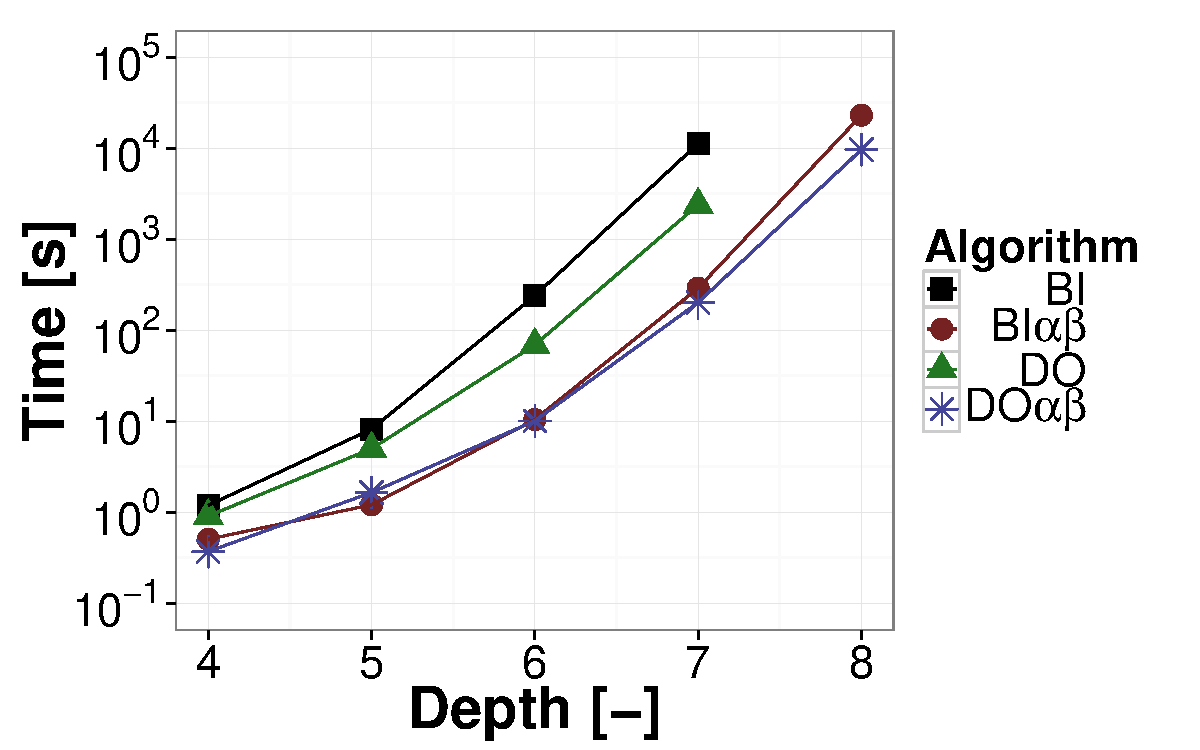
\includegraphics[width=0.5\textwidth]{figures/GS.pdf}
\caption{Comparison of running times on Goofspiel with increasing size of the deck.} \label{fig:off:res:gs}
\end{figure}

Figure~\ref{fig:off:res:gs} depicts the results for the card game Goofspiel (note the logarithmic y-scale).
The results show that a significant number of sub-games has a pure sub-game Nash equilibrium that can be computed using serialized alpha-beta algorithms.
Therefore, the performance of $\biab$ and $\doab$ is fairly similar and the gap only slowly increases in favor of $\doab$ with the increasing size of the game.
Both of these algorithms significantly reduce the number of states visited by the backward induction algorithm (i.e., excluding the number of states evaluated by serialized alpha-beta algorithm).
While \textsc{BI} algorithm evaluates on average more than $32\cdot10^6$ nodes in the setting with $7$ cards in more than $3$ hours, $\biab$ evaluates only $198986$ nodes in less than $5$ minutes. 
The performance is further improved by $\doab$ that evaluates on average $51035$ nodes in less than $4$ minutes.
However, the overhead of the algorithm is slightly higher in case of $\doab$; hence, the difference between $\doab$ and $\biab$ is relatively small in this case.
Finally, the results show that even simple \textsc{DO} algorithm without serialized alpha-beta search can improves the performance of \textsc{BI}.
In the setting with $7$ cards, \textsc{DO} evaluates more than $6\cdot10^6$ nodes which takes on average almost 40 minutes.

The results on Goofspiel highly contrast with the Goofspiel results of the pruning algorithm SMAB presented in \cite{Saffidine12SMAB}.
In their work, the number of evaluated nodes was at best around $20\%$, and the running time improvement was only marginal. 

\begin{figure}
\centering
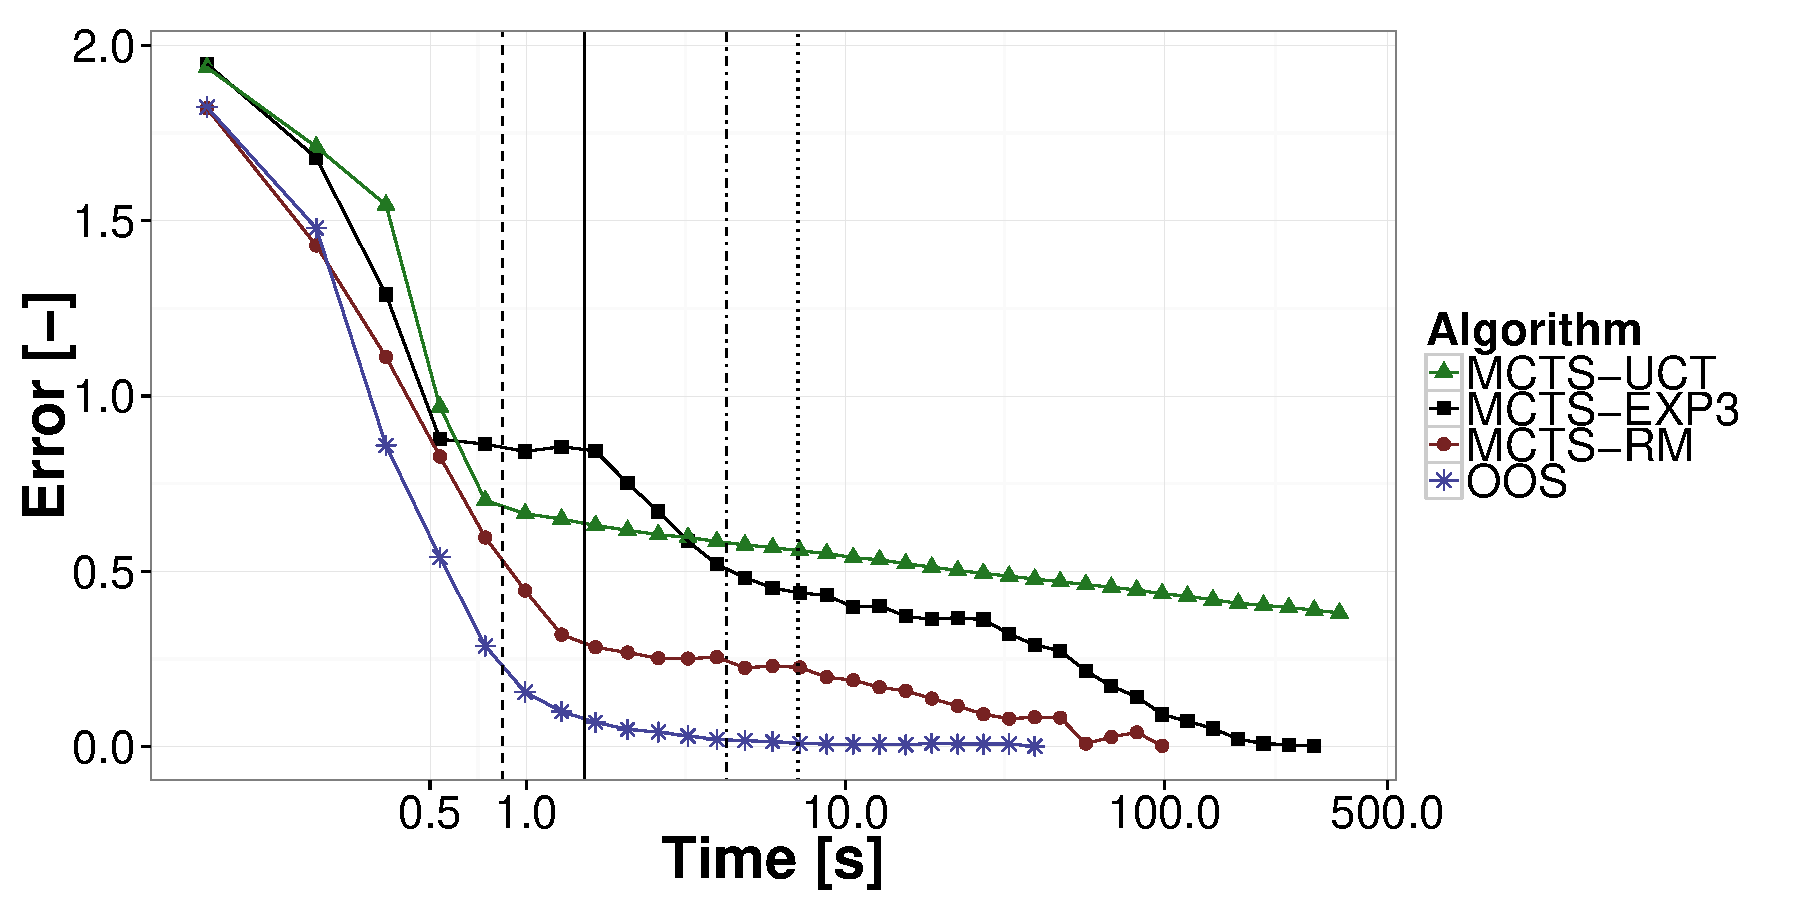
\includegraphics[width=0.85\textwidth]{figures/convergence-gs.pdf}
\caption{Convergence comparison of different sampling algorithms on Goofspiel with $5$ cards. The vertical lines correspond to computation times for exact algorithms.} \label{fig:off:conv:gs}
\end{figure}

Next we focus on the convergence of sampling algorithms -- i.e., their ability to approximate Nash equilibrium strategies of the complete game. 
Figure~\ref{fig:off:conv:gs} depicts the results in this offline settings for Goofspiel game with $5$ cards (note the logarithmic x-scale).
We compare MCTS algorithms with three different selection functions (UCT, EXP3, and RM), and OOS algorithm. 
The results are means out of $20$ runs of each algorithm.
The results show that OOS is the fastest out of all sampling algorithms during the whole time. 
MCTS with Regret Matching selection function is only slightly slower, however, other two selection functions perform worse. 
While EXP3 eventually converges close to $0$, UCT is not able to reach error lower than $0.5$ (the minimum error was $0.37$ out of all runs and all samples).
These results confirm theoretical findings for the algorithms -- convergence is not guaranteed for UCT, and can be expensive (i.e., slow) for EXP3. 
On the other hand, both OOS and RM confirm their quick convergence with is aligned with previous existing results~\cite{}.
The vertical lines represent times for exact algorithms.
In Goofspiel $5$, $\biab$ is slightly faster and finishes first in less than $1$ second, following by $\doab$ ($1.52$ seconds), \textsc{DO} ($4.25$ seconds), and \textsc{BI} ($7.11$).


\subsubsection{Pursuit-Evasion Games}
\begin{figure}
\centering
	\begin{subfigure}{0.49\textwidth}
		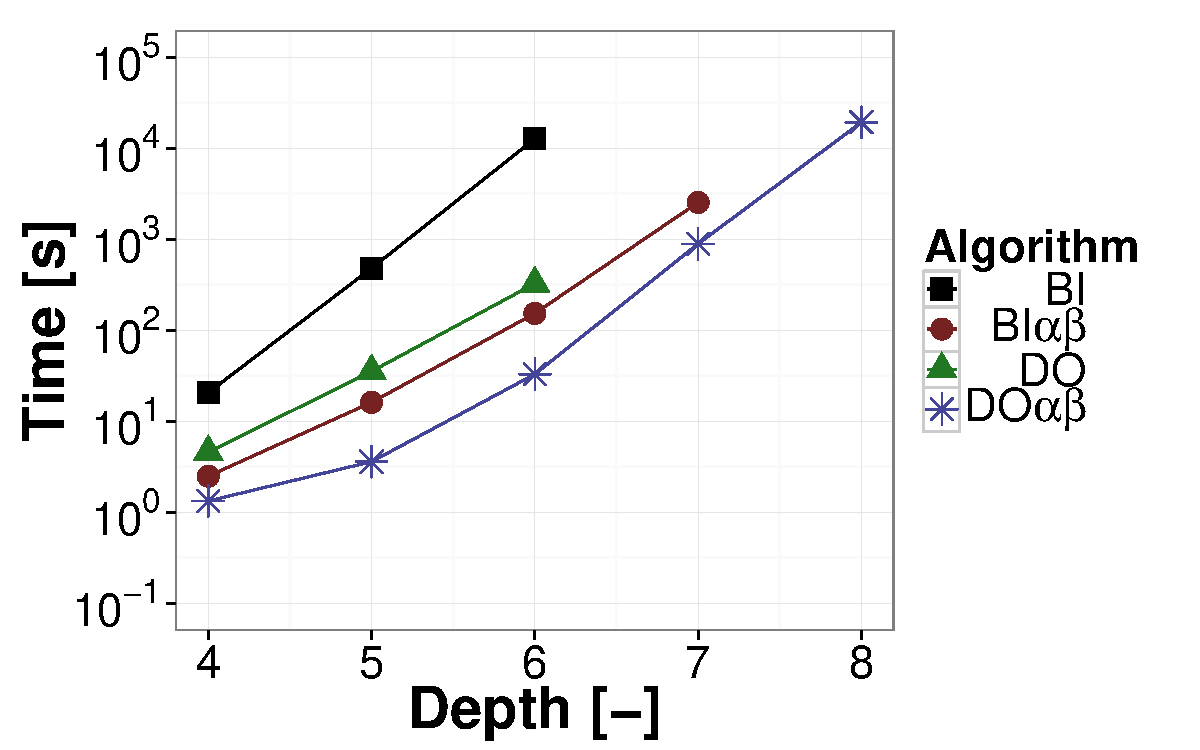
\includegraphics[width=1\textwidth]{figures/PEG4x4.pdf}\caption{}\label{fig:off:res:peg4}
	\end{subfigure}
	\begin{subfigure}{0.49\textwidth}
		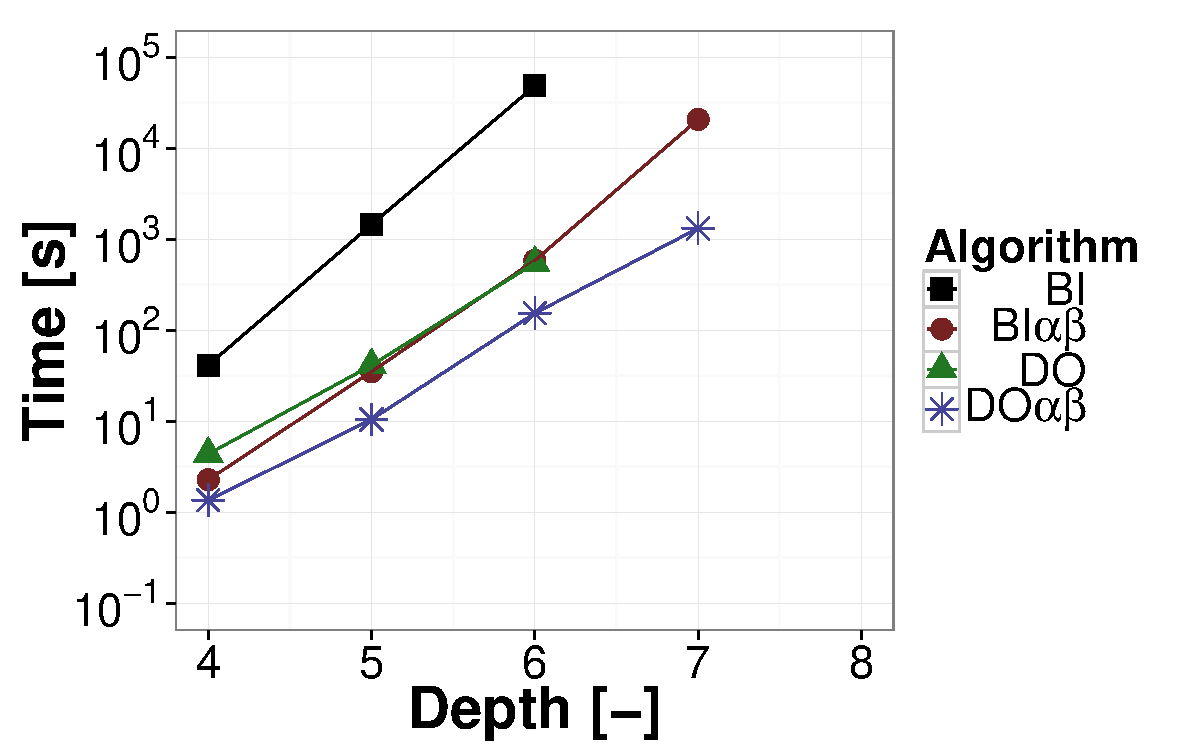
\includegraphics[width=1\textwidth]{figures/PEG5x5.pdf}\caption{}\label{fig:off:res:peg5}
	\end{subfigure}
\caption{Comparison of running times on pursuit-evasion game with increasing number of moves: sub-figure (a) depicts the results on $4\times4$ grid graph, (b) depicts results for $5\times5$ grid.} \label{fig:off:res:peg}
\end{figure}

The results on pursuit-evasion games show more significant improvement when comparing $\doab$ and $\biab$ (see Figure~\ref{fig:off:res:peg}). For both graph the $\doab$ is significantly the fastest. When we compare the performance on graph $5\times5$ with depth set to $6$, \textsc{BI} evaluates more than $49\cdot10^6$ nodes that takes more than $13$ hours. On the other hand, $\biab$ evaluates on average $42001$ nodes taking almost $10$ minutes ($584$ seconds). Interestingly, the benefits of pure integration with alpha-beta search is not that helpful in this game.
This is apparent from results of \textsc{DO} algorithm that evaluates less than $2\cdot10^6$ nodes but it takes slightly over $9$ minutes on average ($547$ seconds). Finally, $\doab$ evaluates only $6692$ nodes and it takes the algorithm less than $3$ minutes.

Large parts of pursuit-evasion game can be solved by serialized alpha-beta algorithms.
These parts typically corresponds to clearly winning, or clearly loosing positions for a player.
However, since there are only two pursuit units, it is still necessary to use mixed strategies for final coordination (capturing the evader close to edge of the graph), and thus mixing strategy occurs near the end of the game tree. 
Therefore, serialized alpha-beta is not able to solve all sub-games, while double-oracle provides additional pruning and cause the improvement in computation time for $\doab$ compared to $\biab$ and all the other algorithms.

\begin{figure}
\centering
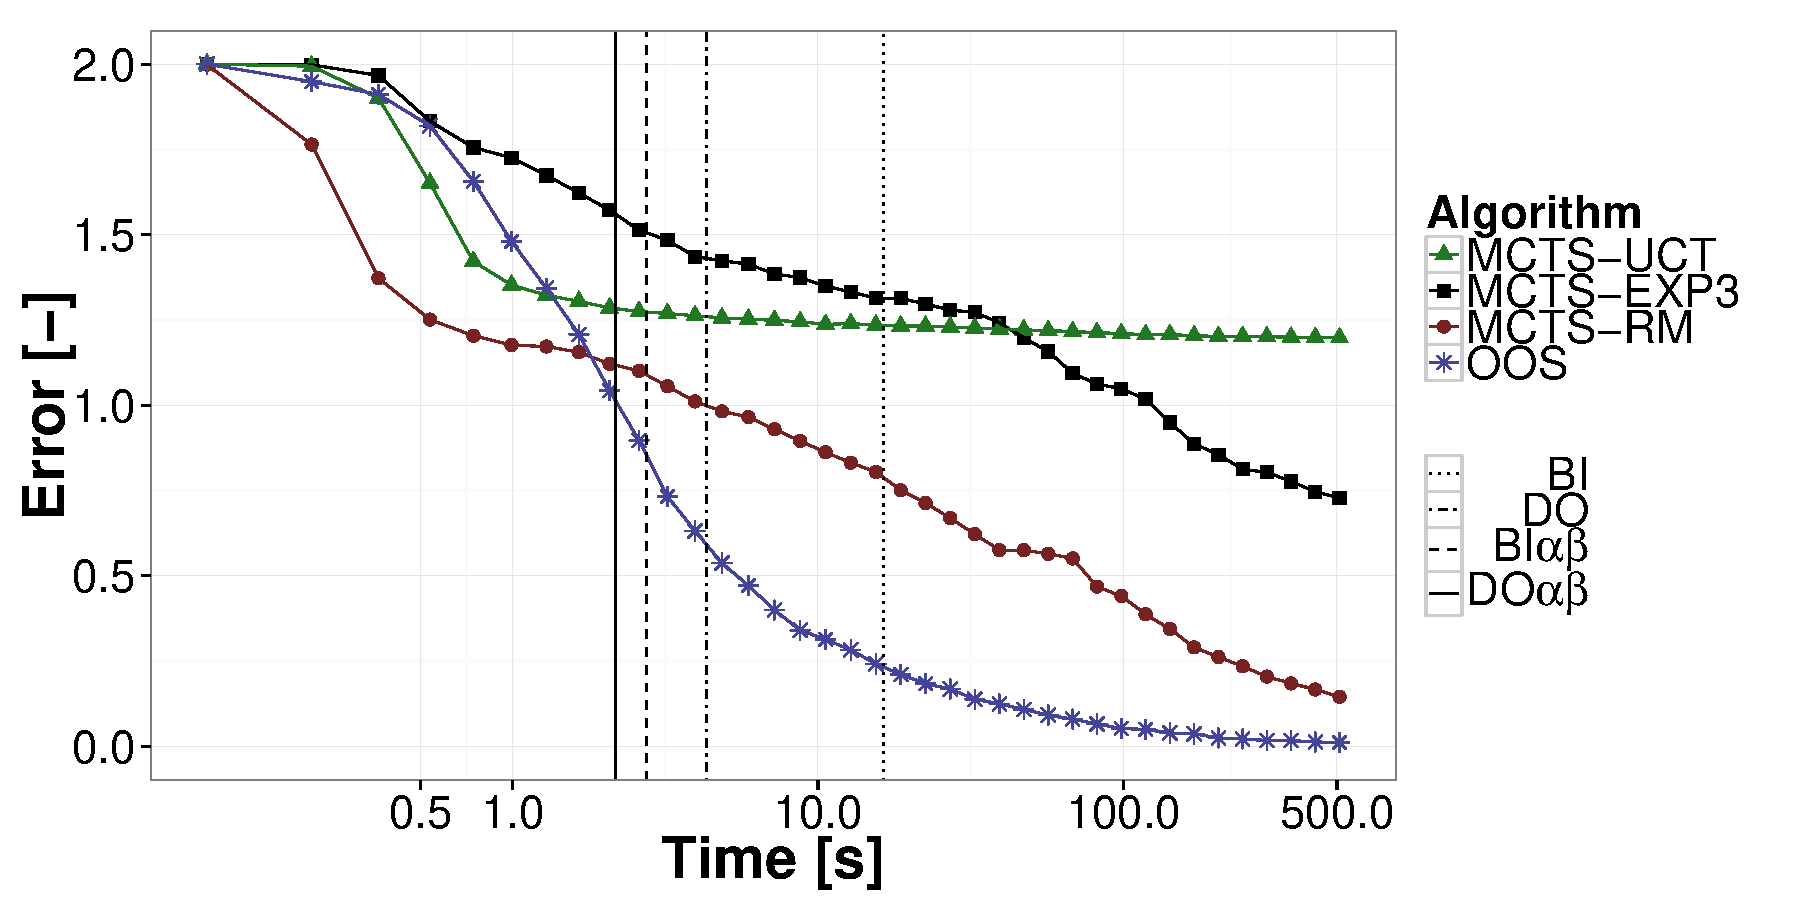
\includegraphics[width=0.85\textwidth]{figures/convergence-peg.pdf}
\caption{Convergence comparison of different sampling algorithms on pursuit-evasion game, on $4\times4$ graph, with depth set to $4$. The vertical lines correspond to computation times for exact algorithms.} \label{fig:off:conv:peg}
\end{figure}

We turn to convergence of the sampling algorithms.
The results are depicted in Figure~\ref{fig:off:conv:peg} for the smaller $4\times4$ graph and $4$ number of moves for each player (note again the logarithmic x-scale).
The results again show that OOS is overall the fastest out of all sampling algorithms, however, during the first iterations both UCT and RM are faster and their exploitability is slightly smaller. 
On the other hand, while OOS is able to keep the convergence rate and reach almost $0$ exploitability, UCT again converges to exploitable strategy with error $0.73$ at best. 
The convergence of RM is much better, however the best final error is $0.13$.
Finally, EXP3 converges even more slowly compared to the goofspiel.
The main difference between the games is the size of the branching factor for the second player (pursuer controls two simultaneously moving units), which can cause more difficulties for the sampling algorithms to estimate good strategies.

As before, the vertical lines represent times for exact algorithms.
In pursuit-evasion game of this setting, $\doab$ is slightly faster and finishes first in $2.77$ seconds, following by $\biab$ ($2.89$ seconds), \textsc{DO} ($5.48$ seconds), and \textsc{BI} ($12.5$).

\subsubsection{Oshi-Zumo}
\begin{figure}
\centering
	\begin{subfigure}{0.49\textwidth}
		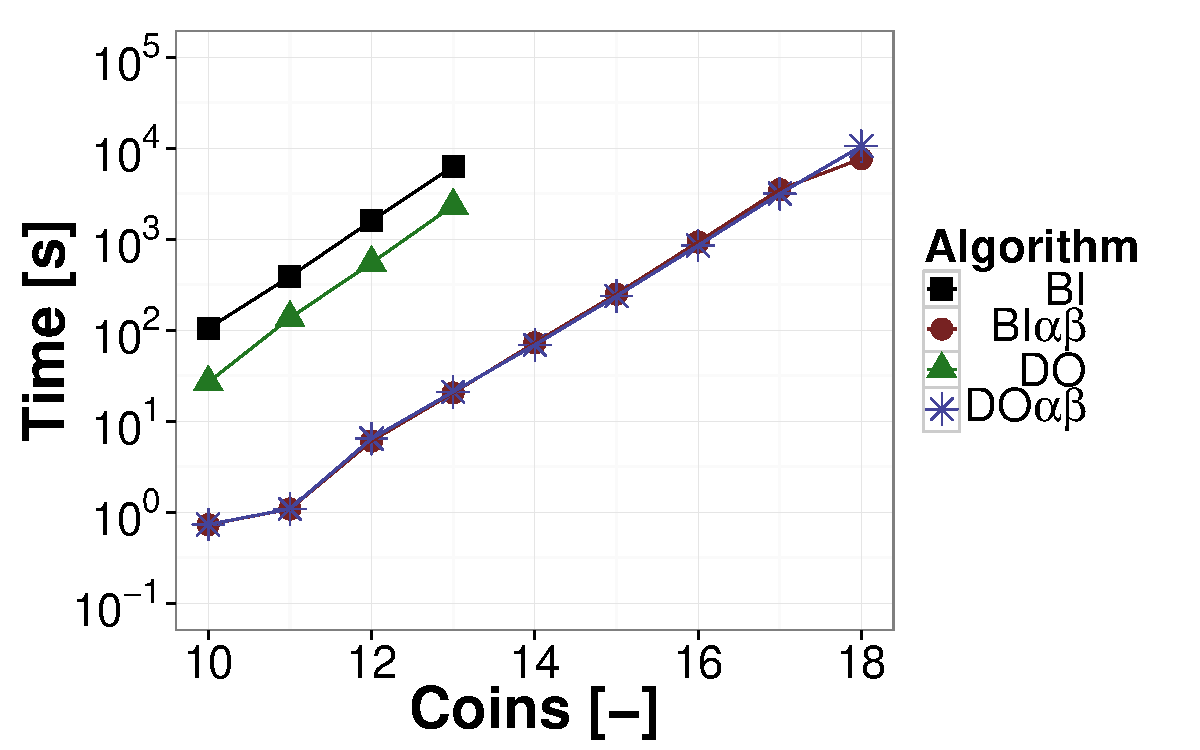
\includegraphics[width=1\textwidth]{figures/OZ-K3.pdf}\caption{}\label{fig:off:res:oz3}
	\end{subfigure}
	\begin{subfigure}{0.49\textwidth}
		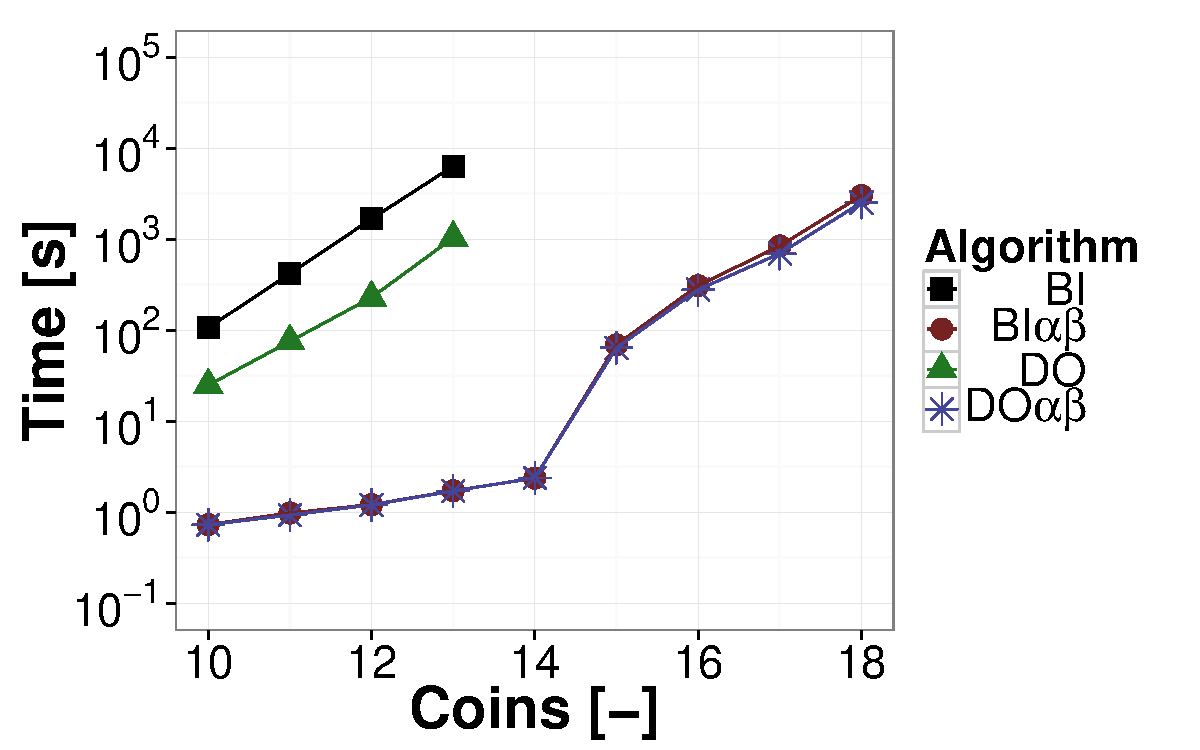
\includegraphics[width=1\textwidth]{figures/OZ-K4.pdf}\caption{}\label{fig:off:res:oz4}
	\end{subfigure}
\caption{Comparison of running times on the Oshi-Zumo game with increasing number of coins: sub-figure (a) depicts the results on with $K$ set to $3$, (b) depicts the results with $K=4$.} \label{fig:off:res:oz}
\end{figure}

Many instances of the Oshi-Zumo game have Nash equilibria in pure strategies. 
Although this does not hold for all the instances, the size of the sub-games with pure NE are rather large and cause dramatic computation speed-up for both algorithms using serialized alpha-beta search.
If the game does not have equilibria in pure strategies, the mixed strategies are still required only near the root node and large end-games are solved using alpha-beta search.
Note that this is different to pursuit-evasion games, where mixed strategies were necessary close to the end of the game tree.
Figure~\ref{fig:off:res:oz} depicts the results for two different setting of the playing field $K$ is either set to $3$ or $4$.
In both cases, the graphs clearly highlights when the whole game does not have an equilibrium in pure strategies -- for $K$ equal to $3$, the change occurs when the number of coins increase from $11$ to $12$, for $K=4$ the first setting with non-pure equilibria is in case with $15$ coins for each player.

The consequence of the advantage of $\biab$ and $\doab$ algorithms that exploit serialized variants of alpha-beta algorihtms is dramatic in Oshi-Zumo game. 
We can see that both \textsc{BI} and \textsc{DO} scale rather badly.
The algorithms were able to scale up to $13$ coins in reasonable time. 
For setting with $K=4$ and $13$ coins, it takes almost $2$ hours for \textsc{BI} to solve the game (the algorithm evaluates $15\cdot10^6$ nodes).
\textsc{DO} improves the performance slightly (the algorithm evaluates nearly $6\cdot10^6$ nodes in $40$ minutes), however, the difference between alpha-beta algorithm is dramatic. 
Both $\biab$ and $\doab$ are in essence solved by executing a single alpha-beta search on each serialization.
Therefore, their performance is identical and it takes $21$ seconds to solve the game.
With an increasing number of coins the algorithms need to find mixed Nash equilibria, however, their performance is in both cases very similar.

\begin{figure}
\centering
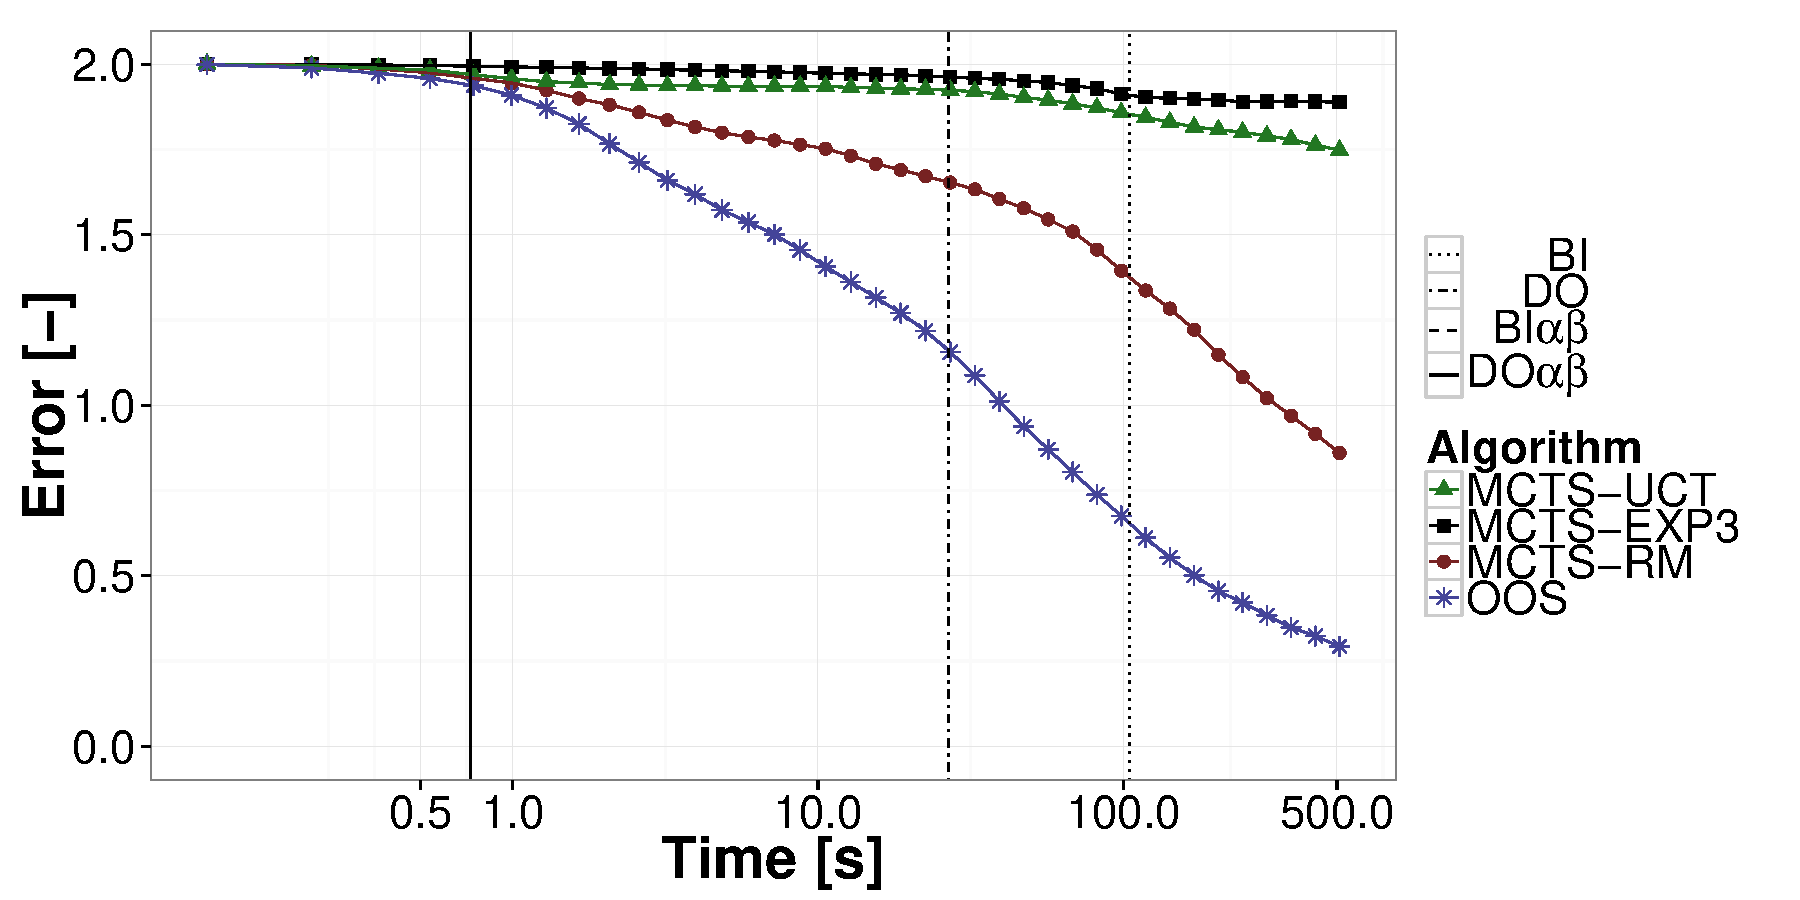
\includegraphics[width=0.85\textwidth]{figures/convergence-oz.pdf}
\caption{Convergence comparison of different sampling algorithms on Oshi-Zumo game, with $10$ coins, $K=3$, and $M=1$. The vertical lines correspond to computation times for exact algorithms.} \label{fig:off:conv:oz}
\end{figure}

Figure~\ref{fig:off:conv:oz} depicts results for convergence of the sampling algorithms for the game with $10$ coins, $K$ set to $3$ and minimum bid set to $1$. This is an easy game for $\doab$ and $\biab$ with pure strategy and both of these algorithms are able to solve the game in less than a second ($0.73$). However, due to large branching factor for both players ($10$ actions at the root node for each player) all sampling algorithms converge extremely slowly. Again, OOS is the best one, however, in a given time limit ($500$ seconds) the algorithm converged to error slightly below $0.5$ ($0.41$). On the other hand, all of the other sampling algorithms perform significantly worse -- RM ends with error slightly over $1$, UCT with $1.78$, and EXP3 with $1.88$.
This confirms our findings from the previous experiment that increasing branching factor slows down the convergence rate.
Secondly, since there is a pure Nash equilibrium, the convergence of the algorithms is also slower since they essentially mix the strategy during the iterations in order to explore the unvisited parts of the game tree. Since none of the sampling algorithms can exploit the fact, their performance in offline solving games like Oshi-Zumo is quite is not compelling.

\subsubsection{Random Games}
In the first variant of the randomly generated games we used games with utility values randomly drawn from a uniform distribution $[0,1]$. 
Such games represent an extreme case, where neither alpha-beta search, nor double-oracle algorithm can save much computation time, since each action can lead to arbitrarily good or bad terminal state. 
In these games, \textsc{BI} algorithm is typically the fastest.
Even though both $\biab$ and $\doab$ evaluate marginally less nodes ($\approx90\%$), the overhead of the algorithms (repeated calculation of alpha-beta algorithm, repeatedly solving linear programs, etc.) causes slower runtime performance in this case.

However, completely random games are rarely instances that need to be solved in practice.
The situation changes, when we use the intuition of good and bad moves and thus add correlation to the utility values.
Figure~\ref{fig:off:res:rg} depicts the results for two different branching factors $4$ and $5$ for each player and increasing depth.
The results show that $\doab$ outperforms all remaining algorithms, although the difference is rather small (still statistically significant).
On the other hand, \textsc{DO} without serialized alpha-beta is not able to outperform \textsc{BI}. 
This is most likely caused by a larger support in mixed sub-game equilibria that cause enumerating most of the actions by the double-oracle algorithm. 
Moreover, this is also demonstrated by the performance of $\biab$ that is only slightly better compared to \textsc{BI}.

The fact that serialized alpha-beta is less successful in randomly generated games is noticeable also when comparing the number of evaluated nodes.
For case with branching factor set to $4$ for both players, and depth $7$, \textsc{BI} evaluates almost $18\cdot10^6$ nodes in almost $3.5$ hours, while $\biab$ evaluates more than $\approx10\cdot10^6$ nodes in almost $3$ hours. 
\textsc{DO} evaluates even more nodes compared to $\biab$ ($\approx12\cdot10^6$) and it is slower compared to both \textsc{BI} and $\biab$. 
Finally, $\doab$ evaluates $\approx2\cdot10^6$ nodes on average and it takes the algorithm slightly over $80$ minutes.

\begin{figure}
\centering
	\begin{subfigure}{0.49\textwidth}
		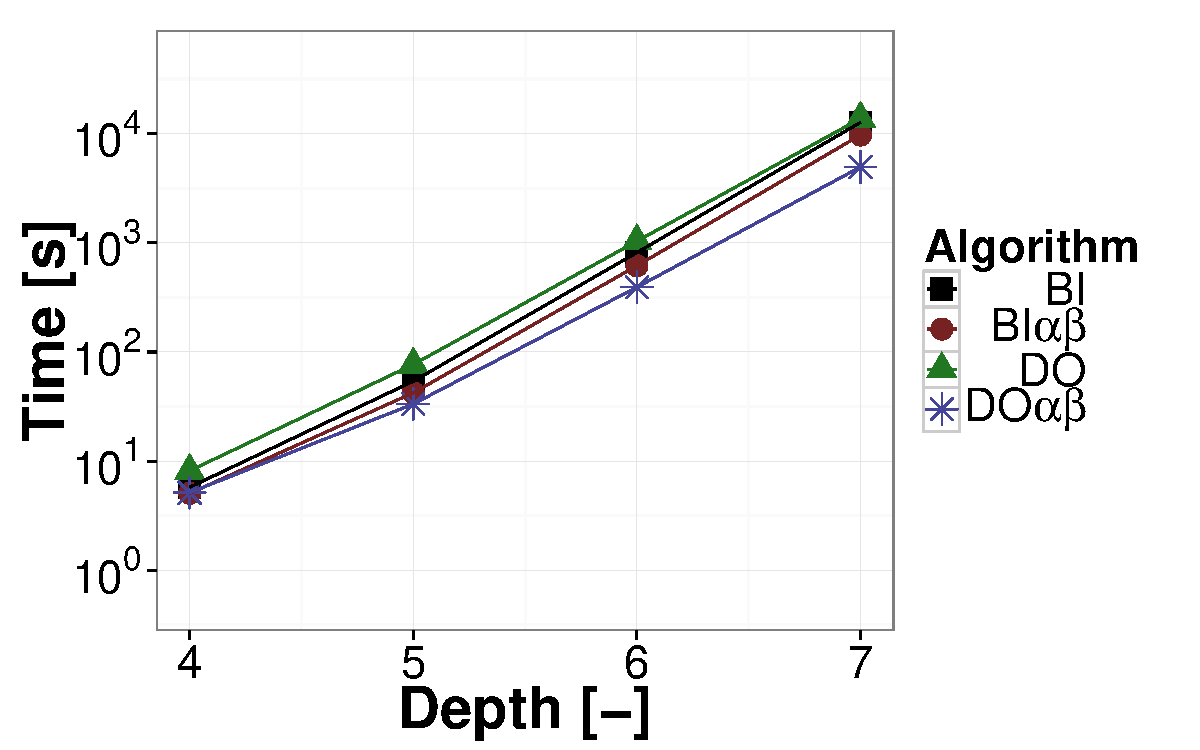
\includegraphics[width=1\textwidth]{figures/RG-BF4-BIN-FALSE.pdf}\caption{}\label{fig:off:res:rgbf4}
	\end{subfigure}
	\begin{subfigure}{0.49\textwidth}
		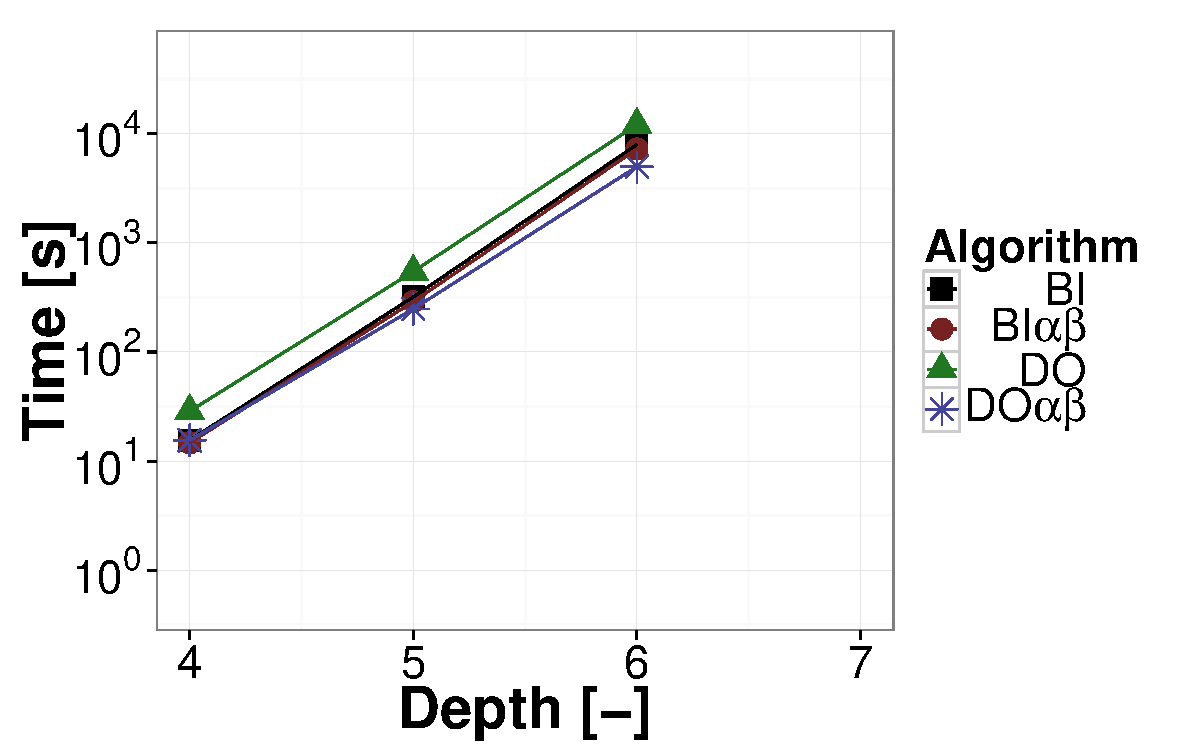
\includegraphics[width=1\textwidth]{figures/RG-BF5-BIN-FALSE.pdf}\caption{}\label{fig:off:res:rgbf5}
	\end{subfigure}
\caption{Comparison of running times on randomly generated games with increasing depth: sub-figure (a) depicts the results with branching factor set to $4$ actions for each player, (b) depicts the results with branching factor $5$.} \label{fig:off:res:rg}
\end{figure}

\begin{figure}
\centering
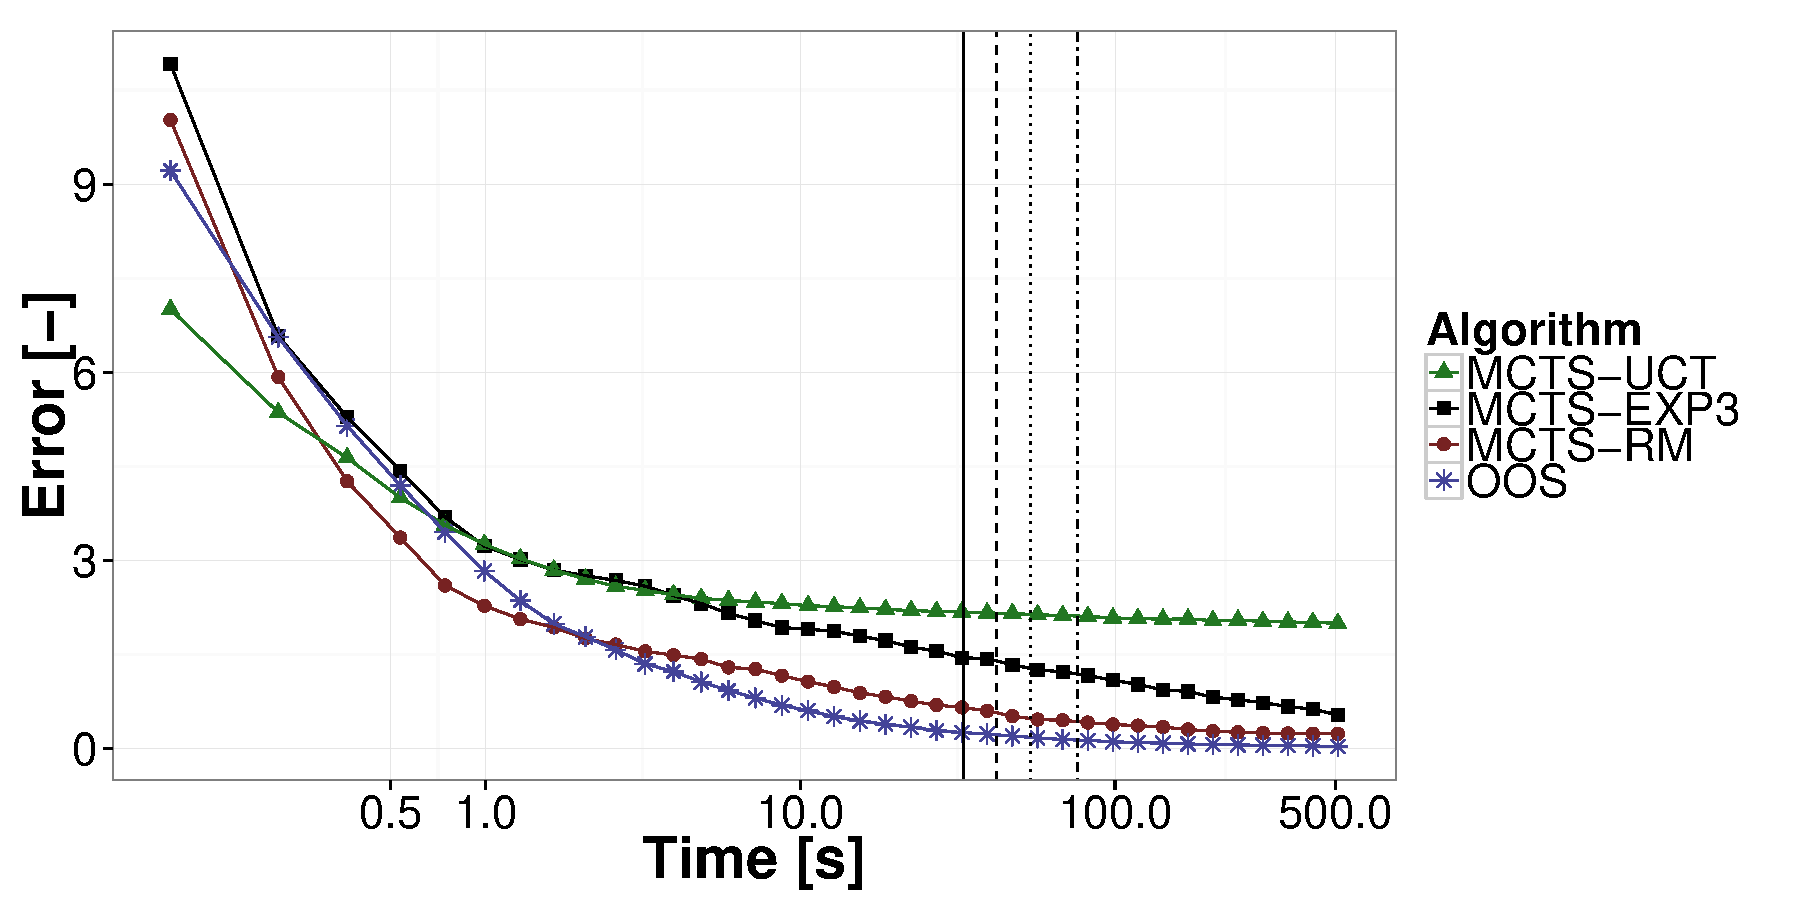
\includegraphics[width=0.85\textwidth]{figures/convergence-rg-fix.pdf}
\caption{Convergence comparison of different sampling algorithms on random game with branching factor $4$ and depth $5$. The vertical lines correspond to computation times for exact algorithms.} \label{fig:off:conv:rg}
\end{figure}

\subsubsection{Tron}
\begin{figure}
\centering
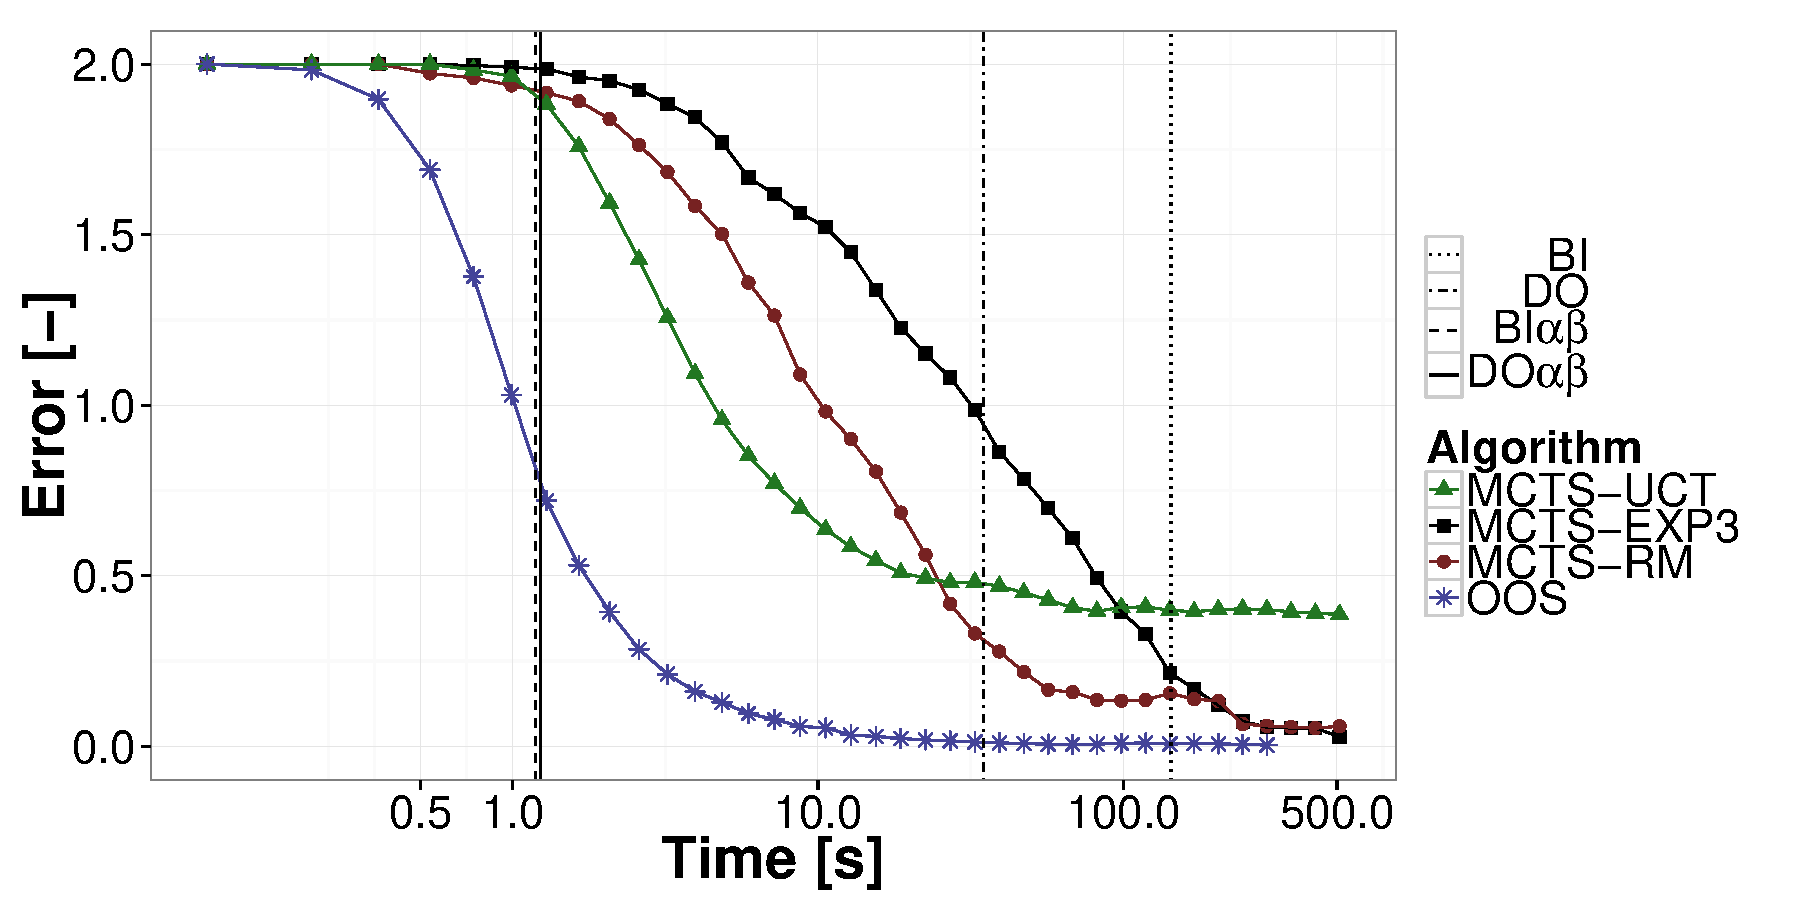
\includegraphics[width=0.85\textwidth]{figures/convergence-tron.pdf}
\caption{Convergence comparison of different sampling algorithms on Tron on grid $5\times6$. The vertical lines correspond to computation times for exact algorithms.} \label{fig:off:conv:rg}
\end{figure}


\subsection{Online Search}

\begin{figure}
\centering
\begin{footnotesize}
\begin{tabular}{|r|rrrrrr|}\hline
Goof&DOAB&OOS&UCT&EXP3&RM&RAND\\\hline
DOAB&49.5(3.2)&35.1(3.0)&25.5(2.8)&13.8(2.2)&18.9(2.5)&91.2(1.8)\\
OOS&61.2(3.1)&51.8(3.2)&47.9(3.2)&42.1(3.1)&47.2(3.2)&70.9(2.9)\\
UCT&71.4(2.9)&52.8(3.2)&50.1(3.2)&52.9(3.1)&49.7(3.2)&61.3(3.1)\\
EXP3&85.2(2.2)&59.2(3.1)&45.8(3.1)&50.9(1.5)&46.9(2.5)&65.6(3.0)\\
RM&78.5(2.6)&56.8(3.1)&48.2(3.1)&55.0(2.5)&51.2(2.8)&62.6(3.1)\\
RAND&8.2(1.8)&28.1(2.9)&39.0(3.1)&30.5(2.9)&37.7(3.1)&51.1(3.2)\\
\hline
\end{tabular}


\begin{tabular}{|r|rrrrrr|}\hline
Oshi&DOAB&OOS&UCT&EXP3&RM&RAND\\\hline
DOAB&49.6(1.4)&93.2(1.5)&92.1(1.7)&91.2(1.7)&89.6(1.9)&99.1(0.6)\\
OOS&11.6(2.0)&54.9(2.9)&51.3(3.0)&50.0(3.0)&34.9(2.8)&98.2(0.8)\\
UCT&8.9(1.8)&54.1(3.0)&51.2(3.0)&51.1(3.0)&35.0(2.8)&97.2(1.0)\\
EXP3&9.0(1.8)&53.5(3.0)&46.9(3.0)&50.6(2.9)&31.6(2.8)&97.9(0.9)\\
RM&10.1(1.8)&72.0(2.6)&64.5(2.9)&69.2(2.7)&51.5(2.9)&99.9(0.1)\\
RAND&0.8(0.6)&3.2(1.1)&3.6(1.1)&1.6(0.8)&1.0(0.6)&49.6(2.9)\\
\hline
\end{tabular}


\begin{tabular}{|r|rrrrrr|}\hline
Rand&DOAB&OOS&UCT&EXP3&RM&RAND\\\hline
DOAB&48.7(2.9)&60.5(2.8)&49.4(2.9)&48.6(2.9)&49.8(2.8)&88.0(1.9)\\
OOS&37.1(2.8)&50.9(2.9)&40.2(2.8)&35.8(2.8)&36.1(2.8)&83.1(2.2)\\
UCT&45.5(2.8)&55.3(2.9)&48.9(2.9)&47.8(2.9)&48.9(2.9)&86.9(2.0)\\
EXP3&48.1(2.8)&61.6(2.8)&49.9(2.9)&47.4(2.8)&49.5(2.8)&91.0(1.6)\\
RM&47.2(2.9)&59.9(2.8)&50.5(2.9)&50.9(2.8)&48.4(2.8)&91.2(1.6)\\
RAND&9.9(1.7)&17.1(2.2)&12.2(1.9)&7.6(1.5)&10.1(1.7)&50.1(2.9)\\
\hline
\end{tabular}

\begin{tabular}{|r|rrrrrr|}\hline
Tron&DOAB&OOS&UCT&EXP3&RM&RAND\\\hline
DOAB&48.7(0.5)&87.4(1.7)&70.0(2.3)&63.4(2.4)&56.9(2.4)&97.9(0.7)\\
OOS&11.1(1.5)&50.6(2.8)&23.2(2.2)&18.7(2.1)&15.1(1.9)&96.0(1.0)\\
UCT&25.4(2.1)&78.1(2.2)&50.0(2.3)&42.0(2.3)&36.0(2.1)&97.8(0.7)\\
EXP3&28.8(2.2)&80.9(2.2)&55.0(2.3)&49.6(2.3)&43.5(2.3)&97.8(0.7)\\
RM&37.4(2.2)&84.9(2.0)&61.6(2.3)&54.6(2.3)&49.0(2.0)&97.7(0.7)\\
RAND&1.4(0.5)&5.0(1.2)&3.5(0.8)&1.9(0.6)&2.4(0.7)&51.1(3.2)\\
\hline
\end{tabular}

\begin{tabular}{|r|rrrrrr|}\hline
TronE&DOAB&OOS&UCT&EXP3&RM&RAND\\\hline
DOAB&28.5(4.7)&58.9(5.7)&49.0(5.3)&44.7(5.3)&41.8(4.7)&97.4(1.8)\\
OOS&40.7(3.8)&50.0(5.0)&45.0(3.8)&45.7(3.8)&43.0(3.3)&94.4(2.5)\\
UCT&47.3(3.9)&52.7(4.6)&50.0(1.3)&45.0(2.4)&46.4(2.4)&98.0(1.6)\\
EXP3&49.0(4.2)&56.0(4.9)&54.7(2.7)&51.0(1.7)&45.9(2.6)&97.7(1.7)\\
RM&52.8(3.9)&59.1(4.7)&53.6(2.6)&52.9(2.2)&50.0(0.0)&98.0(1.6)\\
RAND&3.3(2.0)&4.3(2.9)&1.7(1.4)&1.0(1.1)&2.0(1.6)&47.0(7.7)\\
\hline
\end{tabular}

%\begin{tabular}{|r|rrrrrr|}\hline
%PE1&DOAB&OOS&UCT&EXP3&RM&RAND\\\hline
%DOAB&1.00(0.00)&0.84(0.17)&0.94(0.11)&0.00(0.32)&-0.12(0.31)&0.92(0.12)\\
%OOS&0.16(0.31)&0.94(0.11)&1.00(0.00)&0.72(0.22)&0.74(0.21)&1.00(0.00)\\
%UCT&0.52(0.27)&0.98(0.06)&1.00(0.00)&0.90(0.14)&0.78(0.20)&1.00(0.00)\\
%EXP3&0.38(0.29)&1.00(0.00)&1.00(0.00)&0.80(0.19)&0.70(0.23)&1.00(0.00)\\
%RM&0.76(0.21)&1.00(0.00)&0.96(0.09)&0.88(0.15)&0.78(0.20)&1.00(0.00)\\
%RAND&-0.64(0.24)&0.02(0.32)&0.02(0.32)&-0.86(0.16)&-0.88(0.15)&0.78(0.20)\\\hline
%\end{tabular}
%\begin{tabular}{|r|rrrrrr|}\hline
%PE3&DOAB&OOS&UCT&EXP3&RM&RAND\\\hline
%DOAB&1.00(0.00)&0.76(0.21)&0.26(0.31)&0.08(0.32)&-0.04(0.32)&1.00(0.00)\\
%OOS&-0.06(0.32)&-0.04(0.32)&-0.46(0.28)&-0.66(0.24)&-0.60(0.25)&0.94(0.11)\\
%MCTS-UCT&0.84(0.17)&0.64(0.24)&0.00(0.32)&-0.04(0.32)&-0.28(0.30)&0.96(0.09)\\
%MCTS-EXP3&0.48(0.28)&0.72(0.22)&0.00(0.32)&0.02(0.32)&-0.24(0.31)&1.00(0.00)\\
%MCTS-RM&0.70(0.23)&0.70(0.23)&0.02(0.32)&-0.26(0.31)&-0.26(0.31)&0.98(0.06)\\
%RAND&-1.00(0.00)&-0.90(0.14)&-0.98(0.06)&-1.00(0.00)&-0.98(0.06)&0.30(0.30)\\
%\hline
%\end{tabular}

\begin{tabular}{|r|rrrrrr|}\hline
PE&DOAB&OOS&UCT&EXP3&RM&RAND\\\hline
DOAB&86.1(2.1)&91.7(1.7)&84.3(2.3)&73.0(2.8)&70.4(2.8)&99.3(0.5)\\
OOS&60.2(3.0)&84.1(2.3)&76.2(2.6)&57.3(3.1)&58.8(3.1)&98.5(0.8)\\
UCT&87.5(2.0)&93.2(1.6)&85.4(2.2)&79.9(2.5)&75.3(2.7)&99.0(0.6)\\
EXP3&85.3(2.2)&95.0(1.4)&85.9(2.2)&78.8(2.5)&76.2(2.6)&99.7(0.3)\\
RM&90.0(1.9)&94.9(1.4)&87.1(2.1)&78.5(2.5)&75.2(2.7)&99.2(0.6)\\
RAND&3.1(1.1)&28.3(2.8)&30.8(2.9)&1.6(0.8)&1.5(0.8)&71.0(2.8)\\
\hline
\end{tabular}


\end{footnotesize}
\caption{Goof,PE, Oshi, Rand, Tron with 1000 runs, TronE 150 runs, DOAB with bugs in Good and Tron. TronE with evaluation function. PE from 10 different starts, RG 10 different games. Parameters always OOS:0.6,UCT:2,EXP3:0.2,RM:0.1.}
\end{figure}





